\documentclass{article}

\usepackage{Sweave}
\begin{document}
\Sconcordance{concordance:15_3_20_Loc_results.tex:15_3_20_Loc_results.Rnw:%
1 2 1 1 0 1 1 1 9 6 1 1 2 8 0 1 2 4 1 1 2 8 0 1 2 2 1 1 2 7 0 1 1 6 0 1 %
1 15 0 1 2 1 1 1 2 7 0 1 1 6 0 1 1 15 0 1 2 13 1 1 2 1 0 1 1 4 0 1 2 13 %
1 1 2 1 0 1 1 4 0 1 2 13 1 1 2 1 0 1 1 4 0 1 2 1 1}


\section*{Descriptives}
\subsection*{Amputees}
N=22
Male=15
Female=7
\subsubsection*{Age}
\begin{Schunk}
\begin{Sinput}
> describe(age_amp)
\end{Sinput}
\begin{Soutput}
  vars  n  mean    sd median trimmed   mad min max range  skew kurtosis   se
1    1 22 47.91 13.04   48.5    48.5 14.83  20  67    47 -0.34    -0.98 2.78
\end{Soutput}
\end{Schunk}
\subsection*{Controls}
N=40
Male=30
Female=10
\subsubsection*{Age}
\begin{Schunk}
\begin{Sinput}
> describe(contr_age,na.rm=T)
\end{Sinput}
\begin{Soutput}
  vars  n  mean    sd median trimmed   mad min max range skew kurtosis   se
1    1 39 45.82 13.01     40   45.27 11.86  27  70    43 0.37     -1.4 2.08
\end{Soutput}
\end{Schunk}

\section*{Signficance Tests}
\subsection*{Within Amputees Affected Wrist versus Unaffected Wrist}
\begin{Schunk}
\begin{Sinput}
> describe(wrist_aw)
\end{Sinput}
\begin{Soutput}
  vars n mean   sd median trimmed  mad  min max range skew kurtosis   se
1    1 7 14.9 6.57  10.83    14.9 3.36 8.57  25 16.43  0.4    -1.83 2.48
\end{Soutput}
\begin{Sinput}
> describe(wrist_uw)
\end{Sinput}
\begin{Soutput}
  vars n  mean   sd median trimmed mad   min   max range skew kurtosis   se
1    1 7 15.12 2.89  15.47   15.12   4 12.03 19.93   7.9 0.36    -1.52 1.09
\end{Soutput}
\begin{Sinput}
> t.test(wrist_aw,wrist_uw,paired=T)
\end{Sinput}
\begin{Soutput}
	Paired t-test

data:  wrist_aw and wrist_uw
t = -0.0825, df = 6, p-value = 0.9369
alternative hypothesis: true difference in means is not equal to 0
95 percent confidence interval:
 -6.715630  6.277535
sample estimates:
mean of the differences 
             -0.2190476 
\end{Soutput}
\end{Schunk}

\subsection*{Between Amputees and Controls Unaffected Hand's}
\begin{Schunk}
\begin{Sinput}
> describe(cont_hands)
\end{Sinput}
\begin{Soutput}
  vars  n mean   sd median trimmed mad  min  max range skew kurtosis   se
1    1 40 4.48 1.42   4.19    4.36 1.3 2.03 8.82  6.79 0.84     0.57 0.23
\end{Soutput}
\begin{Sinput}
> describe(amp_hands)
\end{Sinput}
\begin{Soutput}
  vars  n mean   sd median trimmed  mad  min  max range skew kurtosis   se
1    1 20 4.85 1.55   4.47    4.67 1.45 2.98 9.02  6.04 0.96      0.3 0.35
\end{Soutput}
\begin{Sinput}
> t.test(cont_hands,amp_hands)
\end{Sinput}
\begin{Soutput}
	Welch Two Sample t-test

data:  cont_hands and amp_hands
t = -0.8982, df = 35.433, p-value = 0.3752
alternative hypothesis: true difference in means is not equal to 0
95 percent confidence interval:
 -1.2083776  0.4668845
sample estimates:
mean of x mean of y 
 4.478361  4.849107 
\end{Soutput}
\end{Schunk}

\newpage
\subsection*{Correlation: Age and Amputees Unaffected Wrist}
\begin{verbatim}
Pearsons product-moment correlation
data:  x_uw_age and y_uw
t = 0.1375, df = 5, p-value = 0.896
alternative hypothesis: true correlation is not equal to 0
95 percent confidence interval:
 -0.7252079  0.7784482
sample estimates:
       cor 
0.06136081 
\end{verbatim}
\begin{Schunk}
\begin{Sinput}
> plot(age_amp,amp_means[3,]) #plot of age and uw mean loc
> abline(lm(y_aw~x_aw_age), col="red")
\end{Sinput}
\end{Schunk}
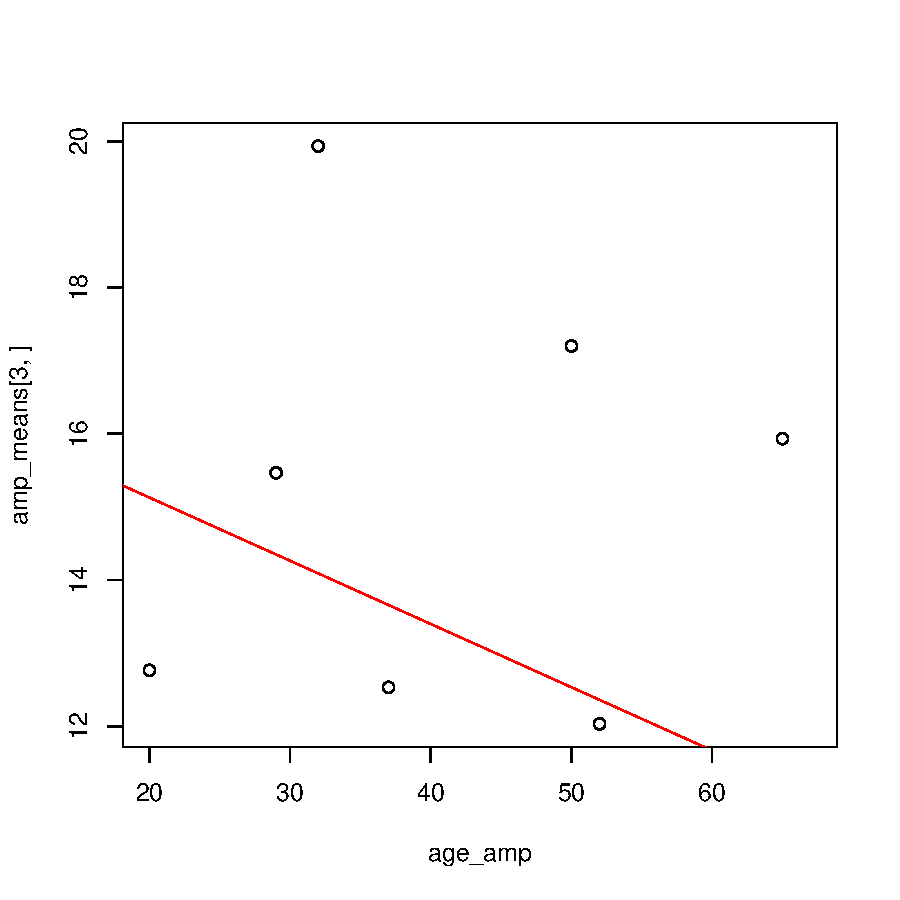
\includegraphics{15_3_20_Loc_results-006}

\newpage
\subsection*{Correlation: Age and Amputees Unaffected Hand}
\begin{verbatim}
Pearsons product-moment correlation
data:  x_uh_age and y_uh
t = 2.0326, df = 18, p-value = 0.05711
alternative hypothesis: true correlation is not equal to 0
95 percent confidence interval:
 -0.01292106  0.73421001
sample estimates:
      cor 
0.4320702
\end{verbatim}
\begin{Schunk}
\begin{Sinput}
> plot(age_amp,amp_means[2,]) #plot of age and uh mean loc
> abline(lm(y_uh~x_uh_age), col="red")
\end{Sinput}
\end{Schunk}
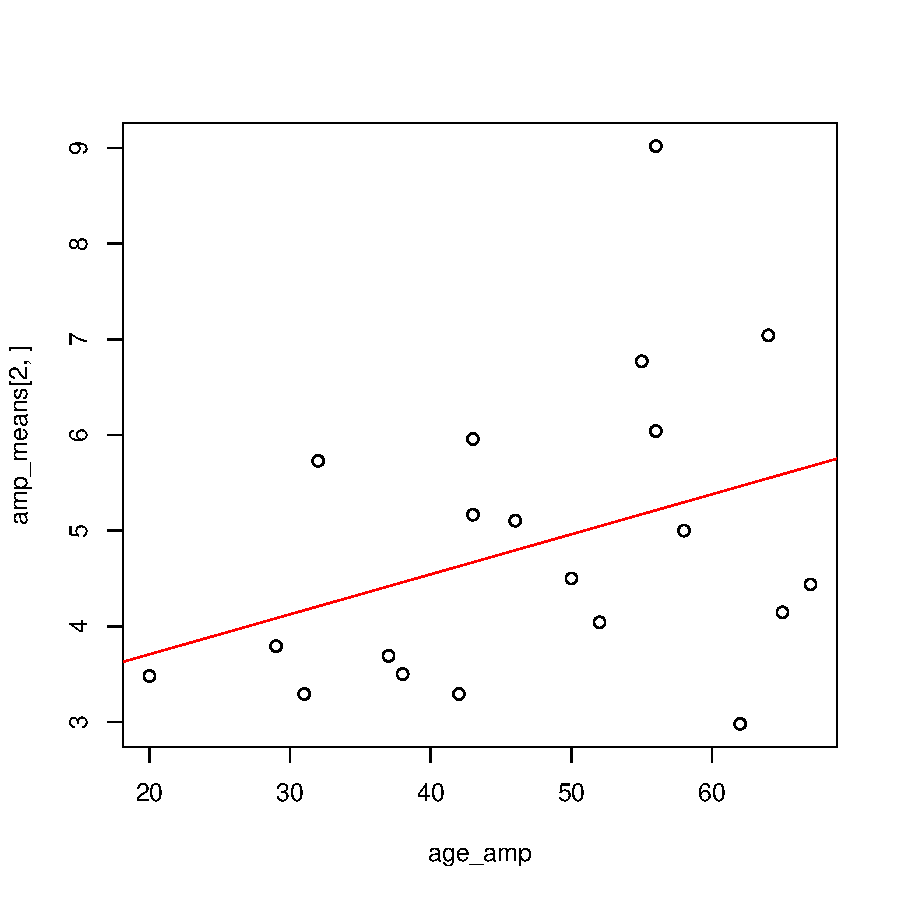
\includegraphics{15_3_20_Loc_results-007}

\newpage
\subsection*{Correlation: Age and Amputees Affected Wrist}
\begin{verbatim}
Pearsons product-moment correlation
data:  x_aw_age and y_aw
t = -0.6766, df = 9, p-value = 0.5157
alternative hypothesis: true correlation is not equal to 0
95 percent confidence interval:
 -0.7242857  0.4376354
sample estimates:
       cor 
-0.2199938 
\end{verbatim}
\begin{Schunk}
\begin{Sinput}
> plot(age_amp,amp_means[3,]) #plot of age and uw mean loc
> abline(lm(y_aw~x_aw_age), col="red")
\end{Sinput}
\end{Schunk}
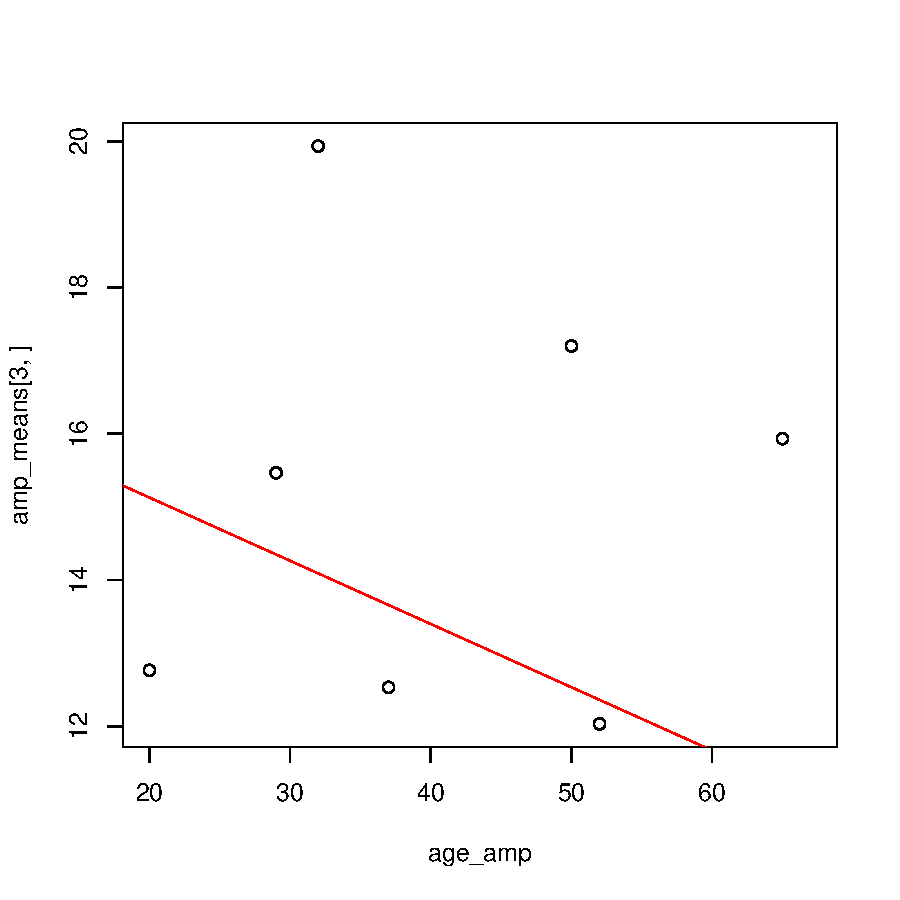
\includegraphics{15_3_20_Loc_results-008}

\end{document}
